\documentclass[11pt,a4paper]{article}
\newcommand{\docname}{Data Card}
\newcommand{\coverdoctype}{DATA CARD}
% Shared preamble for the project sheet and the data card (same look as the report).
\usepackage[T1]{fontenc}
\usepackage[utf8]{inputenc}
\usepackage[english]{babel}
\usepackage{tgtermes}
\usepackage[margin=2.5cm,top=2.6cm,headsep=0.8cm]{geometry}
\usepackage{graphicx}
\usepackage{xcolor}
\usepackage{tikz}
\usepackage{soul}
\usepackage{booktabs}
\usepackage{tabularx}
\usepackage{array}
\usepackage{float}
\usepackage[font=small,labelfont=bf,skip=6pt]{caption}
\usepackage[hidelinks]{hyperref}
\usepackage{enumitem}
\usepackage{microtype}
\usepackage{titlesec}
\usepackage{fancyhdr}

\definecolor{emsigreen}{RGB}{0,191,99}
\definecolor{emsigray}{RGB}{125,125,125}
\sodef\sptext{}{.18em}{.45em}{0em}
\newcommand{\spacedlabel}[1]{\underline{\sptext{#1}}}

\titleformat{\section}{\Large\bfseries}{\thesection.}{0.5em}{}
\titlespacing*{\section}{0pt}{18pt}{8pt}
\setlist{itemsep=2pt,topsep=4pt,leftmargin=1.4em}
\setlength{\parskip}{5pt}
\setlength{\parindent}{0pt}
\newcolumntype{L}{>{\raggedright\arraybackslash}X}
\newcommand{\code}[1]{\texttt{\small #1}}

\pagestyle{fancy}
\fancyhf{}
\fancyhead[L]{\small MedSuperRes Gen --- \docname}
\fancyhead[R]{\small Visual Generative AI, 2026--2027}
\fancyfoot[C]{\small \thepage}
\renewcommand{\headrulewidth}{0.4pt}


\begin{document}
% ------------------------------------------------------------------ Cover page
% Layout reproduces the group's EMSI report template (green bars, EMSI logo, spaced labels).
% All positions are measured from the top-left corner of the A4 page, in cm.
\providecommand{\coverdoctype}{COURSE PROJECT}
\begin{titlepage}
\thispagestyle{empty}
\begin{tikzpicture}[remember picture, overlay, x=1cm, y=-1cm,
                    shift={(current page.north west)}]
  % top-left bar
  \fill[emsigreen] (0, 2.03) rectangle (8.46, 2.49);
  % EMSI logo and the bar under it
  \node[anchor=north west, inner sep=0] at (9.6, 2.67) {
\includegraphics[width=8.3cm]{images/emsi_logo.png}};
  \fill[emsigreen] (8.13, 5.03) rectangle (18.92, 5.54);
  % programme
  \node[anchor=center, align=center, text=emsigray, font=\bfseries\fontsize{15}{19}\selectfont]
       at (13.84, 6.65) {ARTIFICIAL INTELLIGENCE \&\\DATA SCIENCE ENGINEERING};
  \node[anchor=east, font=\small] at (19.55, 7.95) {\underline{ACADEMIC YEAR}};
  \node[anchor=east, font=\normalsize] at (19.93, 8.86) {2026-2027};
  % document type and course
  \node[anchor=center, font=\bfseries\fontsize{30}{34}\selectfont] at (10.5, 10.25) {\coverdoctype};
  \node[anchor=center, align=center, font=\fontsize{13}{17}\selectfont]
       at (10.5, 11.55) {Course: Visual Generative AI};
  % theme
  \node[anchor=west, font=\bfseries\fontsize{15}{18}\selectfont] at (2.67, 13.45) {TOPIC:};
  \fill[emsigreen] (2.92, 13.92) rectangle (18.1, 14.02);
  \node[anchor=north, align=center, text width=15cm, font=\bfseries\fontsize{15.5}{21}\selectfont]
       at (10.5, 14.55) {MedSuperRes Gen: ×4 Super-Resolution of Skin Lesions\\ with SRGAN and Evaluation of Its Utility\\ for Dermatological Classification\\ (DermaMNIST, 32 → 128 px)};
  % right-hand corner bracket
  \fill[emsigreen] (20.47, 16.76) rectangle (21.0, 20.70);
  \fill[emsigreen] (16.86, 20.19) rectangle (21.0, 20.70);
  % left bar and people
  \fill[emsigreen] (2.11, 22.09) rectangle (2.59, 26.97);
  \node[anchor=west, font=\bfseries] at (3.30, 22.86) {\spacedlabel{Prepared by}:};
  \node[anchor=west] at (8.46, 22.86) {Salma Elfataoui \& Wiam Talbi Alami Idrissi};
  \node[anchor=west, font=\bfseries] at (3.30, 24.20) {\spacedlabel{Supervised by}:};
  \node[anchor=west] at (8.46, 24.20) {Prof.\ Oumaima Ouedhiri};
  \node[anchor=west, font=\bfseries] at (3.30, 25.55) {\spacedlabel{Project brief}:};
  \node[anchor=west] at (8.46, 25.55) {No.\ 07 --- MedSuperRes Gen};
\end{tikzpicture}
\end{titlepage}

\setcounter{page}{1}

\section{Overview}

This card documents the data used to train and evaluate the super-resolution models of the
project: where the images come from, how they were split and degraded, what they may and may not
be used for, and the known problems that affect the interpretation of our results.

\begin{table}[H]
\centering\small
\begin{tabularx}{\textwidth}{@{}p{3.3cm}L@{}}
\toprule
Source dataset & DermaMNIST, 128$\times$128 version (MedMNIST+, v3.0) \\
Origin & HAM10000 \cite{tschandl2018}, distributed through MedMNIST \cite{yang2023} \\
Licence & CC BY-NC 4.0 --- non-commercial use only \\
Task & $\times$4 super-resolution (32 $\to$ 128 px); downstream 7-class classification \\
Size & 10{,}015 RGB dermoscopic images, 128$\times$128 px \\
Splits & Official MedMNIST splits: 7{,}007 train / 1{,}003 validation / 2{,}005 test \\
Redistribution & No source image is stored in the repository; \code{src/prepare\_data.py} downloads them \\
\bottomrule
\end{tabularx}
\end{table}

Code, split files and results: \url{https://github.com/salivx/medsuperres-gen}.

% ---------------------------------------------------------------- 1
\section{Composition}\label{sec:comp}

Each image shows one pigmented skin lesion seen through a dermatoscope and carries a single
diagnostic label. Table~\ref{tab:classes} gives the number of images per class and split
(file \code{splits/class\_counts.csv}).

\begin{table}[H]
\centering\small
\caption{Images per class and split.}
\label{tab:classes}
\begin{tabular}{@{}rlrrrr@{}}
\toprule
ID & Class & Train & Val & Test & \% of train \\
\midrule
0 & Actinic keratoses and intraepithelial carcinoma & 228 & 33 & 66 & 3.3 \\
1 & Basal cell carcinoma & 359 & 52 & 103 & 5.1 \\
2 & Benign keratosis-like lesions & 769 & 110 & 220 & 11.0 \\
3 & Dermatofibroma & 80 & 12 & 23 & 1.1 \\
4 & Melanoma & 779 & 111 & 223 & 11.1 \\
5 & Melanocytic nevi & 4{,}693 & 671 & 1{,}341 & 67.0 \\
6 & Vascular lesions & 99 & 14 & 29 & 1.4 \\
\midrule
 & Total & 7{,}007 & 1{,}003 & 2{,}005 & \\
\bottomrule
\end{tabular}
\end{table}

\begin{figure}[H]
\centering
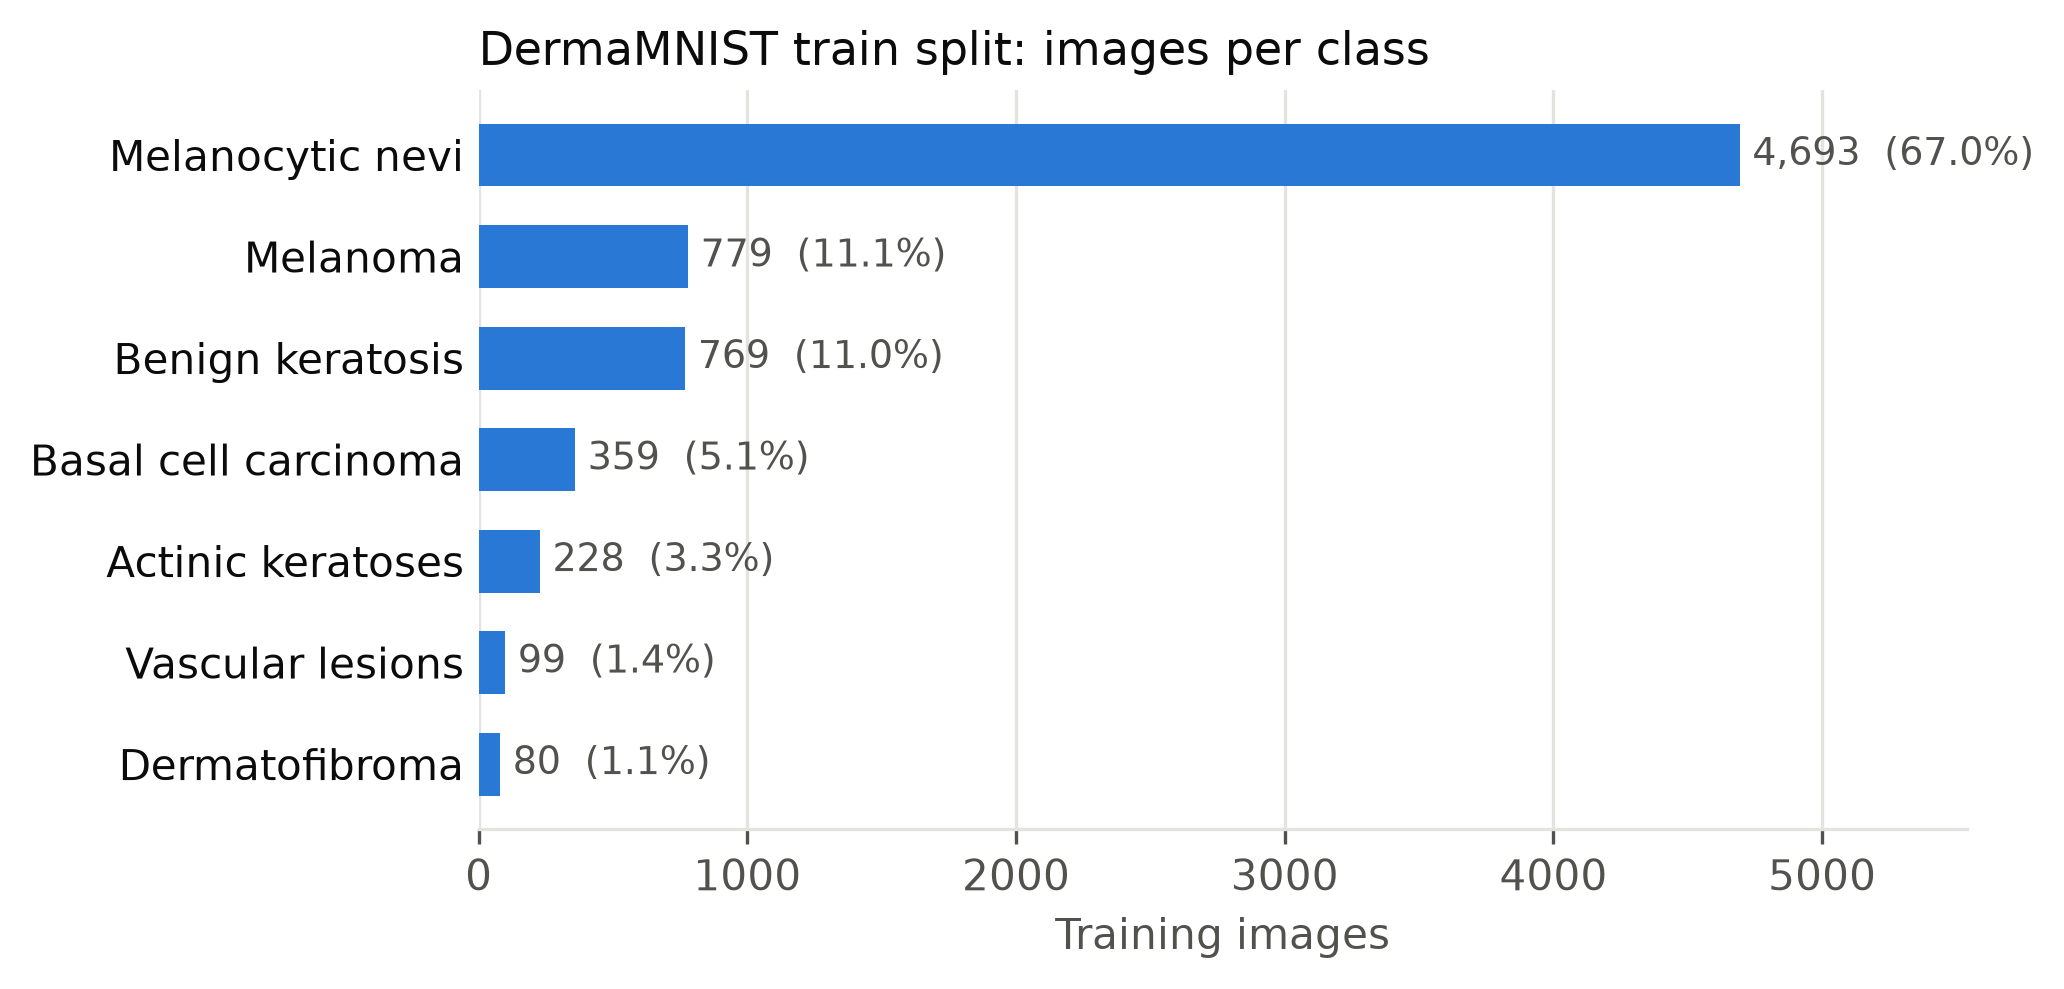
\includegraphics[width=0.72\textwidth]{../figures/data_card/fig1_class_distribution.png}
\caption{Training images per class. Nevi make up two thirds of the training set.}
\label{fig:dist}
\end{figure}

The classes are strongly imbalanced: melanocytic nevi account for 67\% of the training set and
dermatofibroma for 1.1\% (80 images). We therefore report macro F1 and per-class recall rather
than accuracy. With only 23 dermatofibroma and 29 vascular lesions in the test set, the scores of
these two classes vary a lot from one model to another; they are always given with 95\% bootstrap
confidence intervals.

\begin{figure}[H]
\centering
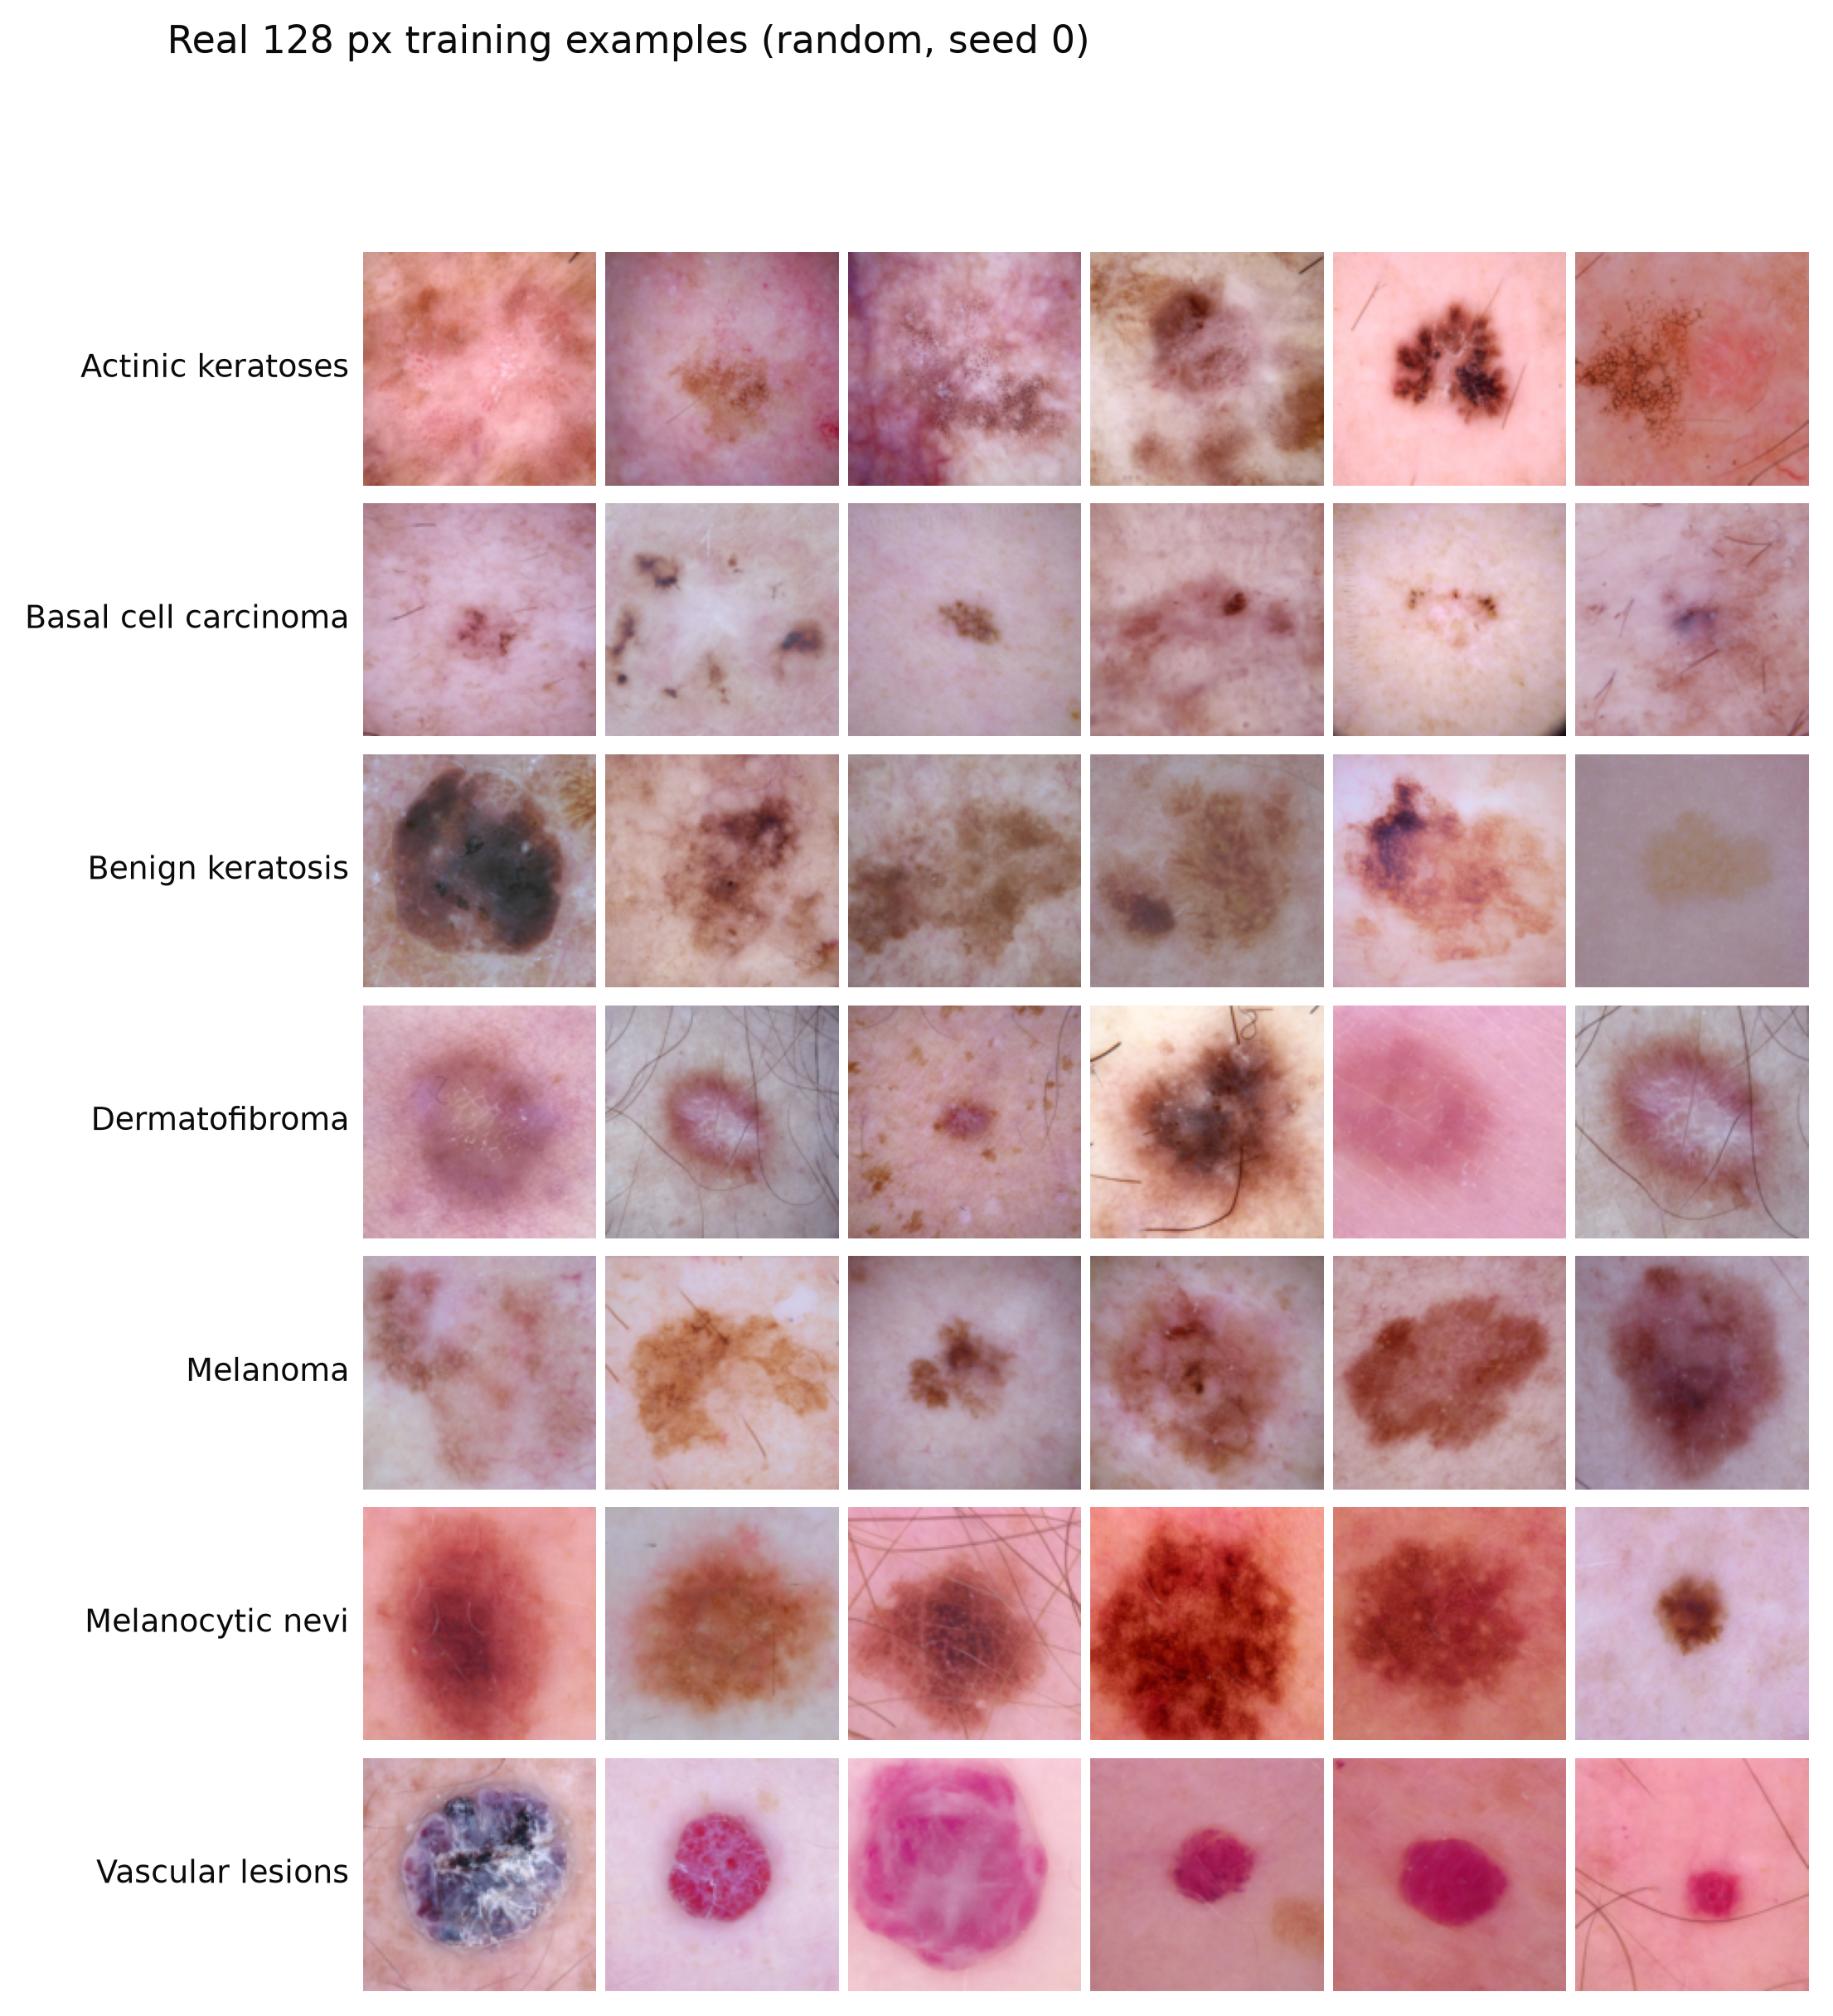
\includegraphics[width=0.52\textwidth]{../figures/data_card/fig2_examples_per_class.png}
\caption{Six random training images per class (seed 0). No test image is shown in this card.}
\label{fig:examples}
\end{figure}

Looking at the images (Fig.~\ref{fig:examples}), hair often crosses the lesion, framing and zoom
change from one image to the next, some images show the dark vignetting of the dermatoscope, and
skin tone and lighting vary. Vascular lesions are easy to recognise by their red colour, whereas
melanoma, nevi and benign keratoses look alike. These are the classes where a super-resolution
model that alters texture is most likely to change a classifier's decision.

% ---------------------------------------------------------------- 2
\section{Splits}

We use the official MedMNIST+ splits without reshuffling them. They are frozen in
\code{splits/train.csv}, \code{val.csv} and \code{test.csv}, which list, for every image, its index,
its label and the SHA-1 hash of the 128~px image; any change in the data changes the hashes and is
therefore detectable. The same files were regenerated on Kaggle and matched the committed ones
image for image.

The training split is used to train the generators and the evaluation classifier. The validation
split is used to select checkpoints and hyperparameters. The test split is used once, after all
training is finished, and never to train, tune or select anything. All figures in this card are
drawn from the training split.

% ---------------------------------------------------------------- 3
\section{Preprocessing and low/high-resolution pairs}

The high-resolution (HR) target is the DermaMNIST 128$\times$128 image as distributed (RGB,
uint8). No image is upsampled to a size above the one available in the data. The 32$\times$32
low-resolution (LR) inputs are computed from the HR image with two degradations, whose exact
parameters are stored in \code{splits/degradation.json} (Table~\ref{tab:degr}, Fig.~\ref{fig:degr}).

\begin{table}[H]
\centering\small
\caption{Degradations used to build the low-resolution inputs.}
\label{tab:degr}
\begin{tabularx}{\textwidth}{@{}p{3.6cm}LL@{}}
\toprule
Degradation & Operations & Parameters \\
\midrule
Bicubic (main) & Bicubic downsampling $\times$4 & PIL \code{Image.BICUBIC} \\
Blur + noise (robustness) & Gaussian blur on the HR image, bicubic $\times$4, additive Gaussian noise
  & blur $\sigma = 1.0$ px; noise $\sigma = 5/255$; seed 2026 \\
\bottomrule
\end{tabularx}
\end{table}

\begin{figure}[H]
\centering
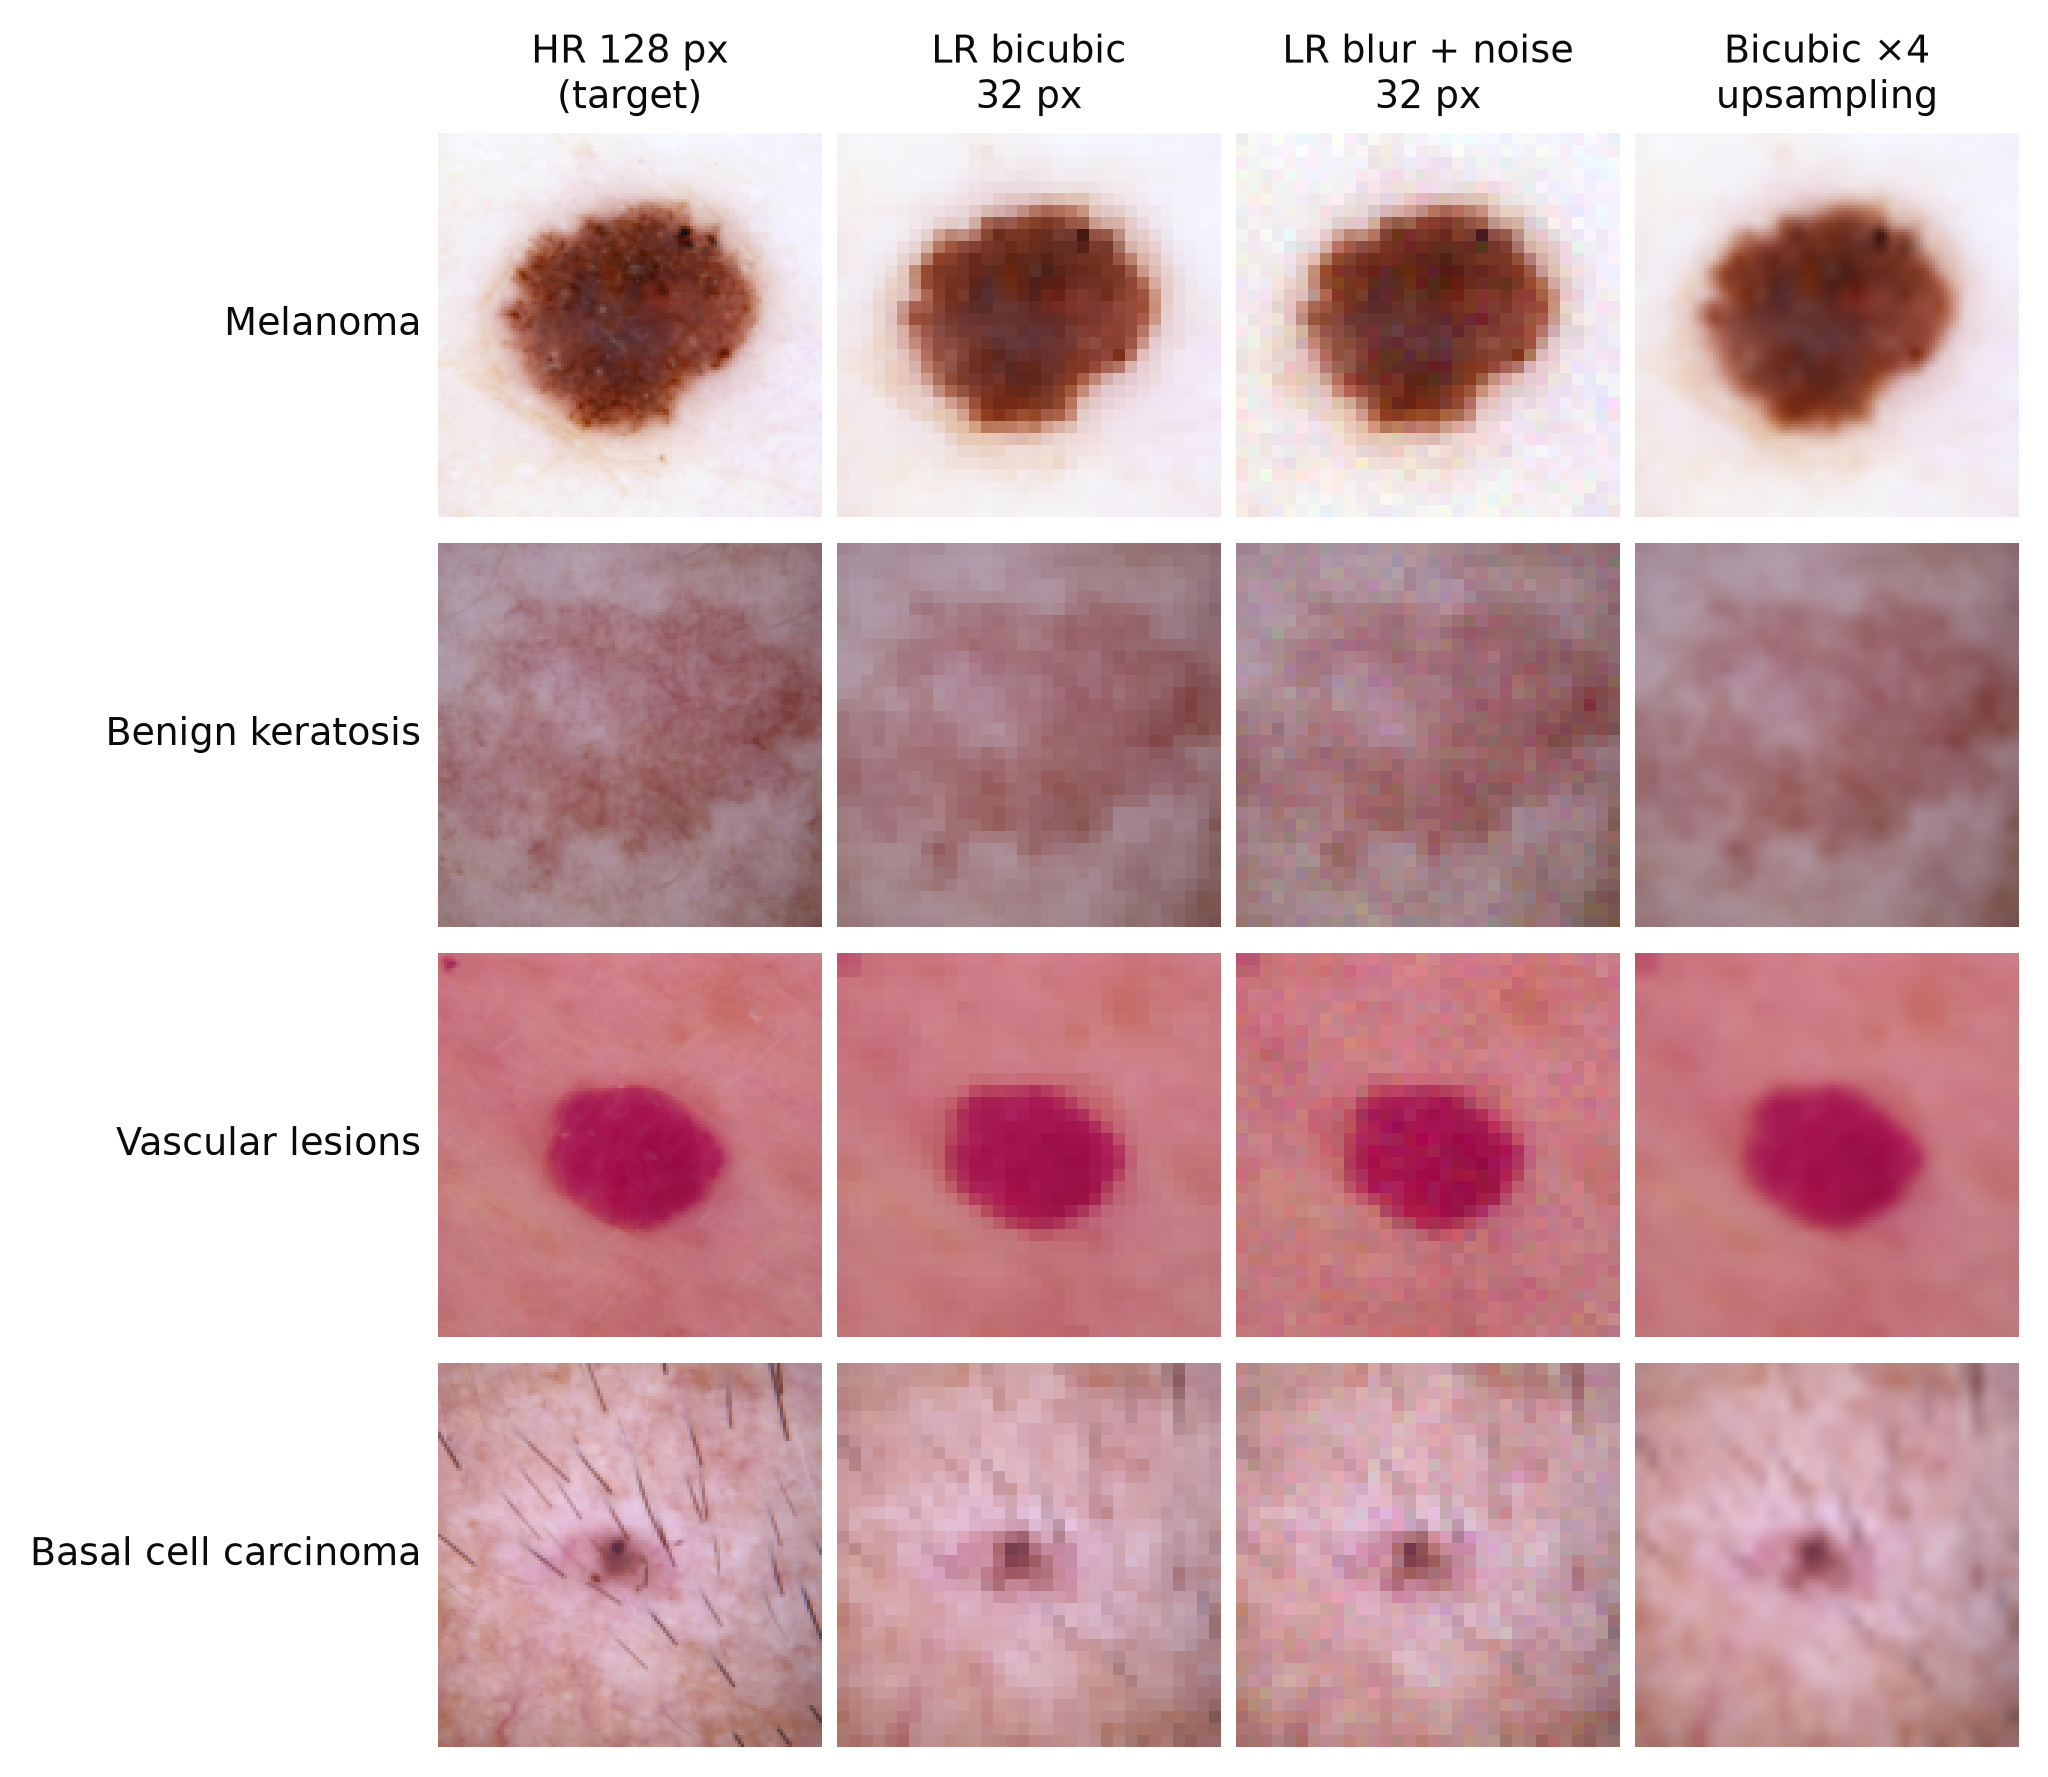
\includegraphics[width=0.62\textwidth]{../figures/data_card/fig3_degradations.png}
\caption{Four training lesions: HR target, the two 32~px inputs (shown with nearest-neighbour
enlargement so that pixels stay visible) and plain bicubic upsampling, the non-learned baseline
that every model has to beat.}
\label{fig:degr}
\end{figure}

{\sloppy The script stores the processed arrays in \code{data/processed/\{split\}.npz} (fields
\code{hr}, \code{lr\_bicubic}, \code{lr\_degraded}, \code{labels}); they are rebuilt on demand and
are not stored in the repository.\par}

% ---------------------------------------------------------------- 4
\section{Intended and out-of-scope use}

The data and the super-resolved images derived from it are meant for research and teaching on
generative super-resolution: measuring how well lesion features survive reconstruction and how
super-resolution affects a classifier.

They must not be used for diagnosis or any clinical decision. Super-resolved images can contain
invented detail --- lesion borders, texture, pigment network, hair --- and are not observations of
the patient. Commercial use is excluded by the licence.

% ---------------------------------------------------------------- 5
\section{Known limitations and biases}

\paragraph{Lesion leakage between splits.} HAM10000 contains 10{,}015 images of 7{,}470 lesions,
and about a quarter of the lesions appear in more than one image. The official DermaMNIST splits
are not made per lesion. Abhishek et al.~\cite{abhishek2025} report 886 images (641 lesions)
shared between train and test, 440 between train and validation and 128 between validation and
test, as well as undetected near-duplicates. We keep the official splits, as the project brief
requires, so absolute test scores may be optimistic. Comparisons between methods remain fair
because they all use the same test set. Corrected versions (DermaMNIST-C and DermaMNIST-E) exist
but are only released at 28 and 224 px.

\paragraph{Labels.} The same authors found mislabelled images in HAM10000 and DermaMNIST. We did
not correct them.

\paragraph{Imbalance.} See Section~\ref{sec:comp}: classes 3 and 6 have very few examples.

\paragraph{Resolution of the target.} The 128~px images are themselves downsampled from the
HAM10000 originals, so the ``ground truth'' of this project is already a reduced image.

\paragraph{Simulated degradation.} The LR inputs are computed, not acquired with a low-resolution
device. Results do not automatically transfer to real low-quality images.

\paragraph{Population.} Patients, devices and skin tones are those of HAM10000; darker skin tones
are under-represented.

% ---------------------------------------------------------------- 6
\section{Reproducing the data}

\begin{verbatim}
pip install -r requirements.txt
python src/prepare_data.py --out data     # download, LR inputs, splits, counts
python src/make_data_card_figures.py      # figures of this card
\end{verbatim}
The SHA-1 hashes in \code{splits/*.csv} make it possible to check that a reproduction recovers
exactly the same images.

% ---------------------------------------------------------------- 7
\section{Authors and AI assistance}

Prepared by Salma Elfataoui and Wiam Talbi Alami Idrissi (EMSI Marrakech, AI \& Data Science
Engineering) for the Visual Generative AI course supervised by Prof.~Oumaima Ouedhiri. The writing
of this card was assisted by Claude (Anthropic); this assistance is also declared in the
repository README, as the project rules require.

\begin{thebibliography}{9}\small
\bibitem{tschandl2018} P.~Tschandl, C.~Rosendahl, H.~Kittler. The HAM10000 dataset, a large
collection of multi-source dermatoscopic images of common pigmented skin lesions.
\emph{Scientific Data}, 5:180161, 2018.
\bibitem{yang2023} J.~Yang et al. MedMNIST v2 --- A large-scale lightweight benchmark for 2D and
3D biomedical image classification. \emph{Scientific Data}, 10:41, 2023.
\bibitem{abhishek2025} K.~Abhishek, A.~Jain, G.~Hamarneh. Investigating the quality of
DermaMNIST and Fitzpatrick17k dermatological image datasets. \emph{Scientific Data}, 2025.
arXiv:2401.14497.
\end{thebibliography}

\end{document}
